\documentclass[11pt,a4paper]{article}

\usepackage[margin=2.3cm, headheight=14pt]{geometry}
\usepackage[T1]{fontenc}
\usepackage[utf8]{inputenc}
\usepackage{lmodern}
\usepackage{amsmath,amssymb}
\usepackage{graphicx}
\graphicspath{{figures/}{assessment/figures/}}
\usepackage{booktabs}
\usepackage{array}
\usepackage{enumitem}
\usepackage{fancyhdr}
\usepackage{hyperref}
\usepackage{xcolor}
\setlength{\parindent}{0pt}
\setlength{\parskip}{0.55em}
\setlength{\emergencystretch}{2.5em}

\hypersetup{
    colorlinks=true,
    linkcolor=blue!60!black,
    urlcolor=blue!60!black,
}

% Right-aligned mark tag on its own line matching UCL COMP0037 coursework style
\newcommand{\qmarks}[1]{\par\nopagebreak\noindent\hfill\mbox{\textbf{[#1 marks]}}}
\newcommand{\qtotal}[1]{\par\smallskip\noindent\hfill\textbf{[Total #1 marks]}\par\medskip}

% UCL-style running footer ("TURN OVER" on odd pages, "CONTINUED" on even pages)
\pagestyle{fancy}
\fancyhf{}
\renewcommand{\headrulewidth}{0pt}
\renewcommand{\footrulewidth}{0.4pt}
\fancyfoot[L]{\thepage}
\fancyfoot[R]{\ifodd\value{page} TURN OVER \else CONTINUED \fi}

\fancypagestyle{endpage}{
    \fancyhf{}
    \renewcommand{\headrulewidth}{0pt}
    \renewcommand{\footrulewidth}{0.4pt}
    \fancyfoot[L]{\thepage}
    \fancyfoot[R]{END OF COURSEWORK}
}

\begin{document}

% --------------------------------------------------------------------------- %
% Title block (emulating COMP0037 2024/25 Coursework 1)
% --------------------------------------------------------------------------- %
\begin{center}
    {\LARGE \textbf{COMP0037 2026/27 Coursework 1}}\\[0.5em]
    {\large COMP0037 Teaching Team}\\[0.3em]
    {\normalsize Term 2, AY 2026/27}
\end{center}

\section*{Overview}
\begin{itemize}[leftmargin=1.5em, itemsep=0.25em]
    \item \textbf{Coursework 01 Release Date:} \textit{TBD (Week 3 / Week 4)}
    \item \textbf{Assignment Due Date:} \textit{TBD (Reading Week --- between Week 5 and Week 6, 16:00 UK time)}
    \item \textbf{Weighting:} 40\% of the module total (Assessment Type: AT10 / GN02 --- Group Coursework with End-Point Submission)
    \item \textbf{Recommended Length:} 2,000--2,500 words per group (excluding figures, tables, equations, references, and appendices)
    \item \textbf{Final Submission Format.} Each group must submit two things:
    \begin{enumerate}[label=\arabic*., leftmargin=1.8em, itemsep=0.2em]
        \item A zip file (which contains the source code implemented to tackle this coursework). The name of the zip file must be of the form \texttt{COMP0037\_CW1\_GROUP\_g.zip}, where \texttt{g} is the letter/number code of your group.
        \item A report in PDF format. It must be named \texttt{COMP0037\_CW1\_GROUP\_g.pdf}.
    \end{enumerate}
    \textit{Note that a penalty of 2\% will be applied if the files are submitted with the wrong name.}
\end{itemize}

\section*{Mark Allocation and Further Instructions}
The total marks for each question are written in the form \textbf{[X marks]}. The coursework is marked out of \textbf{100 marks}. Approximately \textbf{67\%} of the total coursework marks are awarded for your analysis and \textbf{33\%} for your coding of the algorithms. Therefore, please take time and care with your writing, experimental design, and analysis of solutions.

For the submitted code, you must use the notation, variable names, and code structure provided in the lectures and the coursework starter kit (\texttt{cw1\_starter/}, available on Moodle). If you do not use these, we will consider the work a potential plagiarism case and investigate further.

The coursework introduces new robotic environments and tasks distinct from the weekly lab sessions; you will adapt and extend the algorithms learned in Labs 01--05 to solve them. Areas requiring implementation are indicated with \texttt{TODO(CW1-...)} comments.

As discussed in Lecture 00 (Overview), we expect you to take care in writing your report:
\begin{itemize}[leftmargin=1.5em, itemsep=0.2em]
    \item Figures and graphs must be numbered, labelled, and have informative captions.
    \item Equations must be typeset (e.g., via \LaTeX{} or an equation editor). Equations captured by a screenshot from the slides or elsewhere are of low quality and are likely to incur a mark penalty.
    \item When we ask you to write or modify code, provide a clear explanation in your report of what you wrote and why.
    \item Include a \textbf{Reproducibility Block} (exact commands, seeds, Python/PyTorch/MuJoCo versions, and CPU/GPU hardware or Colab runtime) and a \textbf{Signed Group Contribution Table} (Appendix~A, excluded from the word count) documenting each member's primary workstream and peer-verification role.
\end{itemize}

The final mark will be computed by summing all marks awarded on individual questions out of 100. The code will not be independently marked but must be provided before the submission deadline. It may be executed during marking, and if it does not run or fails to reproduce the results presented in the report, this will impact your marks.

\newpage

% --------------------------------------------------------------------------- %
% Use Case
% --------------------------------------------------------------------------- %
\section*{Use Case}
All the questions in this coursework are based on \textbf{MedBot}, an \textbf{Autonomous Hospital Pharmacy and Sterile Laboratory Assistant} operating inside a teaching hospital.

\begin{figure}[htbp]
    \centering
    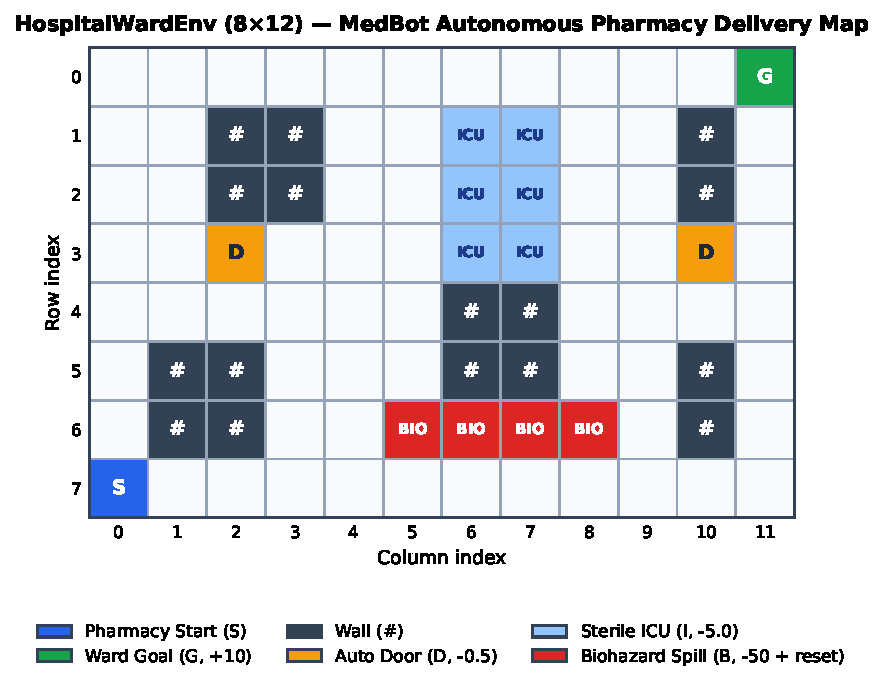
\includegraphics[width=0.92\textwidth]{figures/fig1_hospital_ward.pdf}
    \caption{Overview of the $8\times 12$ hospital ward floor (\texttt{HospitalWardEnv}, defined in \texttt{cw1\_starter/q2\_hospital\_ward.py}). MedBot starts at the pharmacy (\texttt{S}) and must deliver medication to the ward station (\texttt{G}, $+10.0$). Passing through the sterile ICU (\texttt{I}) incurs a $-5.0$ disruption penalty; automatic doors (\texttt{D}) incur $-0.5$; stepping into the biohazard spill (\texttt{B}) incurs $-50.0$ and triggers an immediate decontamination reset to \texttt{S}.}
    \label{fig:hospital_ward}
\end{figure}

MedBot comprises three coupled subsystems:
\begin{enumerate}[label=\arabic*., leftmargin=1.8em, itemsep=0.2em]
    \item \textbf{Dispatch Bay Selector \& Mobile Ward Carrier (Part~1):} Before each delivery run, MedBot selects among $K = 8$ hospital pharmacy dispatch/charging bays (\texttt{q1\_bandits\_hospital.py}) whose service-time rewards are noisy and drift over a hospital shift. It then navigates the $8\times 12$ hospital ward floor (\texttt{HospitalWardEnv}, Figure~\ref{fig:hospital_ward}) with slippery floors, automatic doors, a sterile Intensive Care Unit (ICU) zone, and a biohazard spill.
    \item \textbf{Sterile Biosafety Cabinet 2-DoF Arm (Part~2):} Inside the pharmacy's biosafety cabinet, a 2-DoF planar sample-transfer arm (\texttt{SterileArmEnv}, Figure~\ref{fig:sterile_arm_trolley}a) positions a pipette over sample vials while respecting both hard joint-angle limits and a \textbf{circular keep-out obstacle} representing a fragile benchtop centrifuge.
    \item \textbf{Payload Trolley Physics Digital Twin (Part~2):} MedBot transports tall specimen racks on a wheeled trolley modelled as a new MuJoCo rigid-body system, \texttt{medbot\_payload\_trolley} (Figure~\ref{fig:sterile_arm_trolley}b), whose payload mass, mast hinge damping, and floor friction vary across deliveries.
\end{enumerate}

% --------------------------------------------------------------------------- %
% Part 1
% --------------------------------------------------------------------------- %
\section*{Part 1}
In this part, we examine discrete sequential decision-making under non-stationary uncertainty and tabular model-free reinforcement learning on the hospital ward gridworld.

\begin{enumerate}[label=\textbf{\arabic*.}, leftmargin=1.5em, itemsep=0.6em]

% --- Question 1 ---
\item MedBot must repeatedly select among $K = 8$ pharmacy dispatch/charging bays whose throughput rewards are stochastic (\texttt{cw1\_starter/q1\_bandits\_hospital.py}).
\begin{enumerate}[label=\textbf{\alph*.}, leftmargin=1.6em, itemsep=0.45em]
    \item Define the cumulative regret $R(T)$ of a $K$-armed bandit agent over horizon $T$. Explain why a purely greedy agent ($\varepsilon = 0$) can suffer linear regret $\mathcal{O}(T)$, and explain how \textbf{UCB1} balances exploration and exploitation using Hoeffding's inequality. \qmarks{4}

    \item Complete \texttt{run\_ucb1} in \texttt{q1\_bandits\_hospital.py}. Evaluate $\varepsilon$-greedy ($\varepsilon \in \{0.0, 0.05, 0.1, 0.3\}$) and UCB1 ($c \in \{0.5, 1.0, 2.0\}$) in the \textbf{stationary} regime (\texttt{drift\_std = 0.0}) across horizons $T \in \{200, 1000, 5000\}$ (20 runs each). Present quantitative tables and plots of cumulative regret and percentage of optimal actions, and explain why agent rankings change with horizon $T$. \qmarks{6}

    \item During hospital shift handovers, bay congestion drifts over time (\texttt{drift\_std = 0.05}, where $\mu_a \leftarrow \mu_a + \mathcal{N}(0, 0.05^2)$ at every step). Complete \texttt{run\_epsilon\_greedy\_const\_alpha} in \texttt{q1\_bandits\_hospital.py} using a constant step-size update ($Q_a \leftarrow Q_a + \alpha(r - Q_a)$, $\alpha = 0.1$). Explain your code changes and the mathematical difference between sample-average and exponential recency-weighted updates. \qmarks{6}

    \item Compare sample-average $\varepsilon$-greedy, constant-$\alpha$ $\varepsilon$-greedy, and UCB1 on the \textbf{drifting} hospital bandit (\texttt{drift\_std = 0.05}, $T = 2000$, 20 runs). Discuss qualitatively and quantitatively why UCB1 and sample-average updates degrade under non-stationary rewards. \qmarks{4}
\end{enumerate}
\qtotal{20}

% --- Question 2 ---
\item On freshly disinfected hospital floors, MedBot's wheels slip. As illustrated in Figure~\ref{fig:slip_model}, commanding a nominal direction moves the robot in the intended direction with probability $1 - p_{\mathrm{slip}}$, or into either perpendicular cell with probability $p_{\mathrm{slip}}/2$. Bumping into a wall (\texttt{\#}) or boundary leaves MedBot in its current cell.

\begin{figure}[htbp]
    \centering
    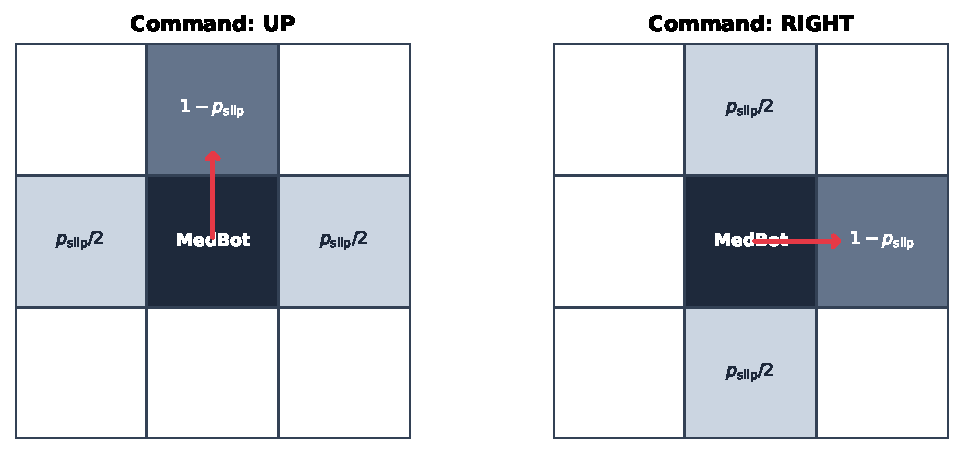
\includegraphics[width=0.72\textwidth]{figures/fig2_slip_model.pdf}
    \caption{Stochastic wheel-slip transition model for MedBot in \texttt{HospitalWardEnv}. The black square denotes the current cell, the red arrow and dark-grey square denote the intended motion (probability $1 - p_{\mathrm{slip}}$), and the light-grey squares denote perpendicular slip outcomes (probability $p_{\mathrm{slip}}/2$ each).}
    \label{fig:slip_model}
\end{figure}

\begin{enumerate}[label=\textbf{\alph*.}, leftmargin=1.6em, itemsep=0.45em]
    \item Write the Bellman optimality equation for $Q^*(s, a)$ and contrast the TD target used by \textbf{Q-Learning} (off-policy) with that of \textbf{SARSA} (on-policy). State the theoretical conditions under which tabular Q-Learning converges to $Q^*$. \qmarks{4}

    \item Complete \texttt{train\_tabular} in \texttt{cw1\_starter/q2\_hospital\_ward.py} to implement both Q-Learning and SARSA on \texttt{HospitalWardEnv} ($\gamma = 0.95$, 800 episodes). Run a controlled sweep over wheel slip $p_{\mathrm{slip}} \in \{0.0, 0.1, 0.2, 0.4\}$ (at $\varepsilon = 0.1$) and over exploration rate $\varepsilon \in \{0.05, 0.1, 0.25\}$ (at $p_{\mathrm{slip}} = 0.2$). Present learning curves and rendered policies for each regime. \qmarks{8}

    \item Analyse how the optimal path changes across $p_{\mathrm{slip}}$ and $\varepsilon$ relative to the sterile ICU (\texttt{I}), automatic doors (\texttt{D}), and biohazard spill (\texttt{B}). Explain qualitatively and quantitatively why SARSA selects a more conservative corridor around \texttt{B} than Q-Learning during training, and identify the slip threshold where both algorithms abandon the lower corridor entirely. \qmarks{6}
\end{enumerate}
\qtotal{18}

\newpage

% --------------------------------------------------------------------------- %
% Part 2
% --------------------------------------------------------------------------- %
\section*{Part 2}
In this part, we move from discrete tables to neural function approximation, dual-barrier continuous safe control (CBFs), and GPU-batched physics simulation for sim-to-real robustness.

\begin{figure}[htbp]
    \centering
    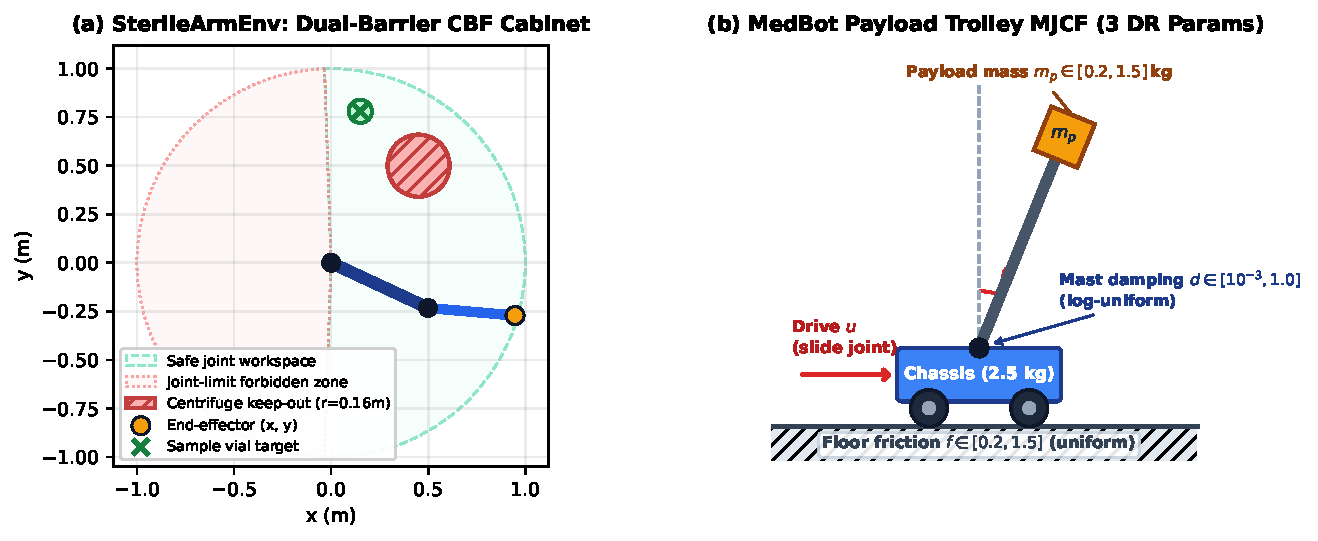
\includegraphics[width=\textwidth]{figures/fig3_sterile_arm_trolley.pdf}
    \caption{Part~2 MedBot subsystems: (a)~\texttt{SterileArmEnv} (\texttt{q3\_sterile\_arm.py}), a 2-DoF planar sample-transfer arm operating inside a biosafety cabinet with hard joint limits and an internal circular centrifuge keep-out zone ($r = 0.16\,$m); (b)~mechanical schematic of \texttt{medbot\_payload\_trolley} (\texttt{q4\_payload\_sim.py}), showing the wheeled chassis ($2.5\,$kg), slide actuator $u$, hinged specimen mast ($\theta$), and the three randomized physical parameters ($m_p$, $d$, $f$).}
    \label{fig:sterile_arm_trolley}
\end{figure}

% --- Question 3 ---
\item Inside the pharmacy's biosafety cabinet, the 2-DoF arm (\texttt{cw1\_starter/q3\_sterile\_arm.py}) must reach sample vials on the far side of a fragile centrifuge without violating joint limits ($q_i \in [-1.6, 1.6]\,$rad) or allowing the end-effector to enter the centrifuge keep-out disk ($\|\mathrm{FK}(q) - c_{\mathrm{obs}}\|_2 < 0.16\,$m).
\begin{enumerate}[label=\textbf{\alph*.}, leftmargin=1.6em, itemsep=0.45em]
    \item Explain Sutton's \textbf{Deadly Triad} and describe the role of (i)~the experience replay buffer, (ii)~the decoupled target network, and (iii)~Huber (\texttt{smooth\_l1}) loss in stabilising DQN. Why must time-limit truncations bootstrap while true task terminations set $d = 1$? \qmarks{5}

    \item Adapt your DQN agent from the labs to run on \texttt{SterileArmEnv(mode="discrete")} and implement \textbf{Double DQN} (selecting the greedy next action with the online network $Q_\theta$ and evaluating it with the target network $Q_{\theta^-}$). Explain your implementation and why Double DQN mitigates value overestimation. \qmarks{6}

    \item Run a multi-seed comparison (3 seeds, 300 episodes) of standard DQN, Double DQN, and an ablation without a target network on \texttt{SterileArmEnv(mode="discrete")}. Compare learning curves, greedy success rate, centrifuge collision rate, and joint chattering (mean total $|\Delta q_1| + |\Delta q_2|$ per episode). Discuss the limitations of discrete action spaces when navigating around tight workspace obstacles. \qmarks{7}

    \item Complete \texttt{cbf\_safety\_shield} in \texttt{q3\_sterile\_arm.py} to project nominal continuous velocities $u_{\mathrm{nom}}$ so that \textbf{both} constraints hold: (i)~joint-angle limits $q_{\min} \le q + u\,\Delta t \le q_{\max}$ and (ii)~the circular centrifuge barrier $h_{\mathrm{obs}}(q) = \|\mathrm{FK}(q) - c_{\mathrm{obs}}\|_2^2 - r_{\mathrm{obs}}^2 \ge 0$ via the discrete-time CBF condition $\nabla h_{\mathrm{obs}}(q)^\top u\,\Delta t + \alpha_{\mathrm{obs}} h_{\mathrm{obs}}(q) \ge 0$ using \texttt{jacobian(q)}. Also implement a \textbf{soft-penalty A2C baseline} (negative reward on limit or obstacle hits, without the shield). Explain your implementation. \qmarks{6}

    \item Compare three continuous A2C configurations on \texttt{SterileArmEnv(mode="continuous")} over 500 episodes (3 seeds): (i)~Unshielded A2C, (ii)~Soft-Penalty A2C, and (iii)~Dual-Barrier CBF-Shielded A2C. Evaluate mean return, cumulative joint-limit violations, and cumulative centrifuge collisions. Explain the \textit{limit-parking} pathology and why soft penalties cannot guarantee zero collisions during exploration whereas the CBF shield does. \qmarks{8}
\end{enumerate}
\qtotal{32}

% --- Question 4 ---
\item Before deploying MedBot's wheeled specimen trolley in hospital corridors, the engineering team benchmarks simulation throughput and quantifies payload-tipping uncertainty using the new MJCF model \texttt{medbot\_payload\_trolley} in \texttt{cw1\_starter/q4\_payload\_sim.py}.
\begin{enumerate}[label=\textbf{\alph*.}, leftmargin=1.6em, itemsep=0.45em]
    \item Explain why simulating $N = 1$ world on GPU (MuJoCo Warp) is substantially slower than single-core CPU MuJoCo, and identify the hardware mechanisms (SIMT parallelism, CUDA-Graph capture via \texttt{wp.ScopedCapture}, and fixed-size contact buffers \texttt{nconmax}/\texttt{njmax}) that enable GPU throughput to surpass CPU at high \texttt{nworld}. \qmarks{4}

    \item Benchmark \texttt{trolley\_model()} on CPU MuJoCo and GPU MuJoCo Warp across \texttt{nworlds} $\in \{1, 2, 4,$ $8, 16, 32, 64, 128, 256\}$ (state your exact CPU and GPU hardware or Colab runtime). Plot total steps/s and per-world steps/s against the CPU baseline, and identify the exact hardware crossover \texttt{nworld}. \qmarks{5}

    \item Complete \texttt{sample\_trolley\_randomization} in \texttt{q4\_payload\_sim.py} to randomize all three physical parameters across batched worlds: (i)~\texttt{mast\_damping} $\in [10^{-3}, 1.0]$ (supporting both \textbf{linear-uniform} and \textbf{log-uniform} modes), (ii)~\texttt{floor\_friction} $\in [0.2, 1.5]$, and (iii)~\texttt{payload\_mass} $\in [0.2, 1.5]\,$kg. Explain how each parameter is written into the batched MuJoCo Warp model. \qmarks{6}

    \item Run $N = 32$ parallel open-loop rollouts from identical initial mast tilt ($\theta_0 = +0.25\,$rad, 500 steps) comparing narrow vs.\ wide randomization ranges and linear vs.\ log-uniform damping. Quantify the terminal tilt spread $\sigma_{\mathrm{final}}$ and justify mathematically why dissipative parameters such as hinge damping require log-uniform sampling ($p(d) \propto 1/d$). \qmarks{5}
\end{enumerate}
\qtotal{20}

% --- Question 5 ---
\item The hospital now intends to deploy the continuous \texttt{SterileArmEnv} policy onto a \textbf{physical 2-DoF benchtop pipetting arm} inside a real biosafety cabinet where joint friction varies by $\pm 40\%$ with sterilisation cycles and joint encoders exhibit bounded measurement noise of $|\hat{q}_i - q_i| \le 0.03\,$rad.
\begin{enumerate}[label=\textbf{\alph*.}, leftmargin=1.6em, itemsep=0.45em]
    \item Describe, \textbf{but do not implement}, an end-to-end training and deployment pipeline combining \textbf{Actor-Critic with GAE}, \textbf{Dual-Barrier CBF safety shielding}, and \textbf{GPU-batched Domain Randomization}. Your answer must explicitly address:
    \begin{enumerate}[label=(\roman*), leftmargin=1.8em, itemsep=0.15em]
        \item how both the joint-limit margin and the circular centrifuge radius $r_{\mathrm{obs}}$ must be inflated to preserve safety under bounded encoder noise $|\hat{q}_i - q_i| \le 0.03\,$rad (show how encoder error maps to end-effector position uncertainty via the manipulator Jacobian);
        \item which dynamics parameters should be randomized during training and with what probability distributions; and
        \item what quantitative validation checks you would execute in simulation and on the bench before enabling full-speed actuation near glass vials.
    \end{enumerate} \qmarks{10}
\end{enumerate}
\qtotal{10}

\end{enumerate}

\bigskip
\begin{center}
    \textbf{[Coursework 1 Total: 100 marks]}
\end{center}

\section*{Getting Help}
You are encouraged to use the Moodle assignment discussion forum when you get stuck. Please check the forum regularly and help answer each other's questions. If you have questions about this coursework, please post them on the forum rather than emailing the teaching team directly, so that all groups can see the reply.

\section*{Submission and Feedback}
The deadline for submission is \textbf{16:00 UK time} on the due date specified on Moodle. Late penalties will start to accrue if any element of the submission (report PDF or source-code ZIP) has a receipt time of 16:01 or later, following UCL's standard AT10/GN02 late-submission policy:
\begin{itemize}[leftmargin=1.5em, itemsep=0.15em]
    \item $< 2$ working days late: 10 percentage points deduction;
    \item $2$--$5$ working days late: capped at pass;
    \item $> 5$ working days late: mark of 1.00\% / Grade E.
\end{itemize}

\newpage
\thispagestyle{endpage}
\section*{Appendix A: Mandatory Group Contribution \& Reproducibility Template}
Include a completed version of the table below at the end of your report PDF (excluded from the word count). Every technical question (Q1--Q4) must have both a \textbf{Primary Lead} and a \textbf{Peer Verifier} (a different group member who independently ran the submitted code to confirm reproducibility).

\begin{table}[htbp]
    \centering
    \renewcommand{\arraystretch}{1.35}
    \begin{tabular}{@{} >{\raggedright\arraybackslash}p{2.4cm} >{\raggedright\arraybackslash}p{1.8cm} >{\raggedright\arraybackslash}p{4.8cm} >{\raggedright\arraybackslash}p{4.0cm} >{\raggedright\arraybackslash}p{1.5cm} @{}}
        \toprule
        \textbf{Student Name} & \textbf{UCL ID} & \textbf{Primary Workstream(s) \& Code Modified} & \textbf{Peer-Verification Role \& Report Sections} & \textbf{Sign-off} \\
        \midrule
        Member 1 & & e.g., Q1 (\texttt{q1\_bandits\_hospital.py}) & Verified Q2 code; Q5 synthesis & \\
        Member 2 & & e.g., Q2 (\texttt{q2\_hospital\_ward.py}) & Verified Q3 code; Q5 synthesis & \\
        Member 3 & & e.g., Q3 (\texttt{q3\_sterile\_arm.py}) & Verified Q4 code; Q5 synthesis & \\
        Member 4 & & e.g., Q4 (\texttt{q4\_payload\_sim.py}) & Verified Q1 code; Q5 synthesis & \\
        \bottomrule
    \end{tabular}
    \caption{Group contribution and peer-verification sign-off table (adapt to 3 rows for 3-student groups).}
\end{table}

\end{document}
